

\tikzset{every picture/.style={line width=0.75pt}} %set default line width to 0.75pt        

\begin{tikzpicture}[x=0.75pt,y=0.75pt,yscale=-1,xscale=1]
%uncomment if require: \path (0,319); %set diagram left start at 0, and has height of 319

%Shape: Rectangle [id:dp5853281871424232] 
\draw  [color={rgb, 255:red, 0; green, 128; blue, 2 }  ,draw opacity=1 ][line width=3.75]  (10.8,134.17) -- (330.77,134.17) -- (330.77,255) -- (10.8,255) -- cycle ;
%Shape: Rectangle [id:dp0668476806187166] 
\draw  [color={rgb, 255:red, 116; green, 73; blue, 156 }  ,draw opacity=1 ][line width=3.75]  (10.77,9.84) -- (330.44,9.84) -- (330.44,129) -- (10.77,129) -- cycle ;
%Shape: Rectangle [id:dp8412963857367168] 
\draw  [color={rgb, 255:red, 179; green, 0; blue, 2 }  ,draw opacity=1 ][line width=3.75]  (335.52,9.84) -- (655.19,9.84) -- (655.19,129) -- (335.52,129) -- cycle ;
%Shape: Rectangle [id:dp403011712811292] 
\draw  [color={rgb, 255:red, 192; green, 89; blue, 161 }  ,draw opacity=1 ][line width=3.75]  (335.75,134.09) -- (655.42,134.09) -- (655.42,255) -- (335.75,255) -- cycle ;
%Image [id:dp4663100234222186] 
\draw (135.5,43.75) node  {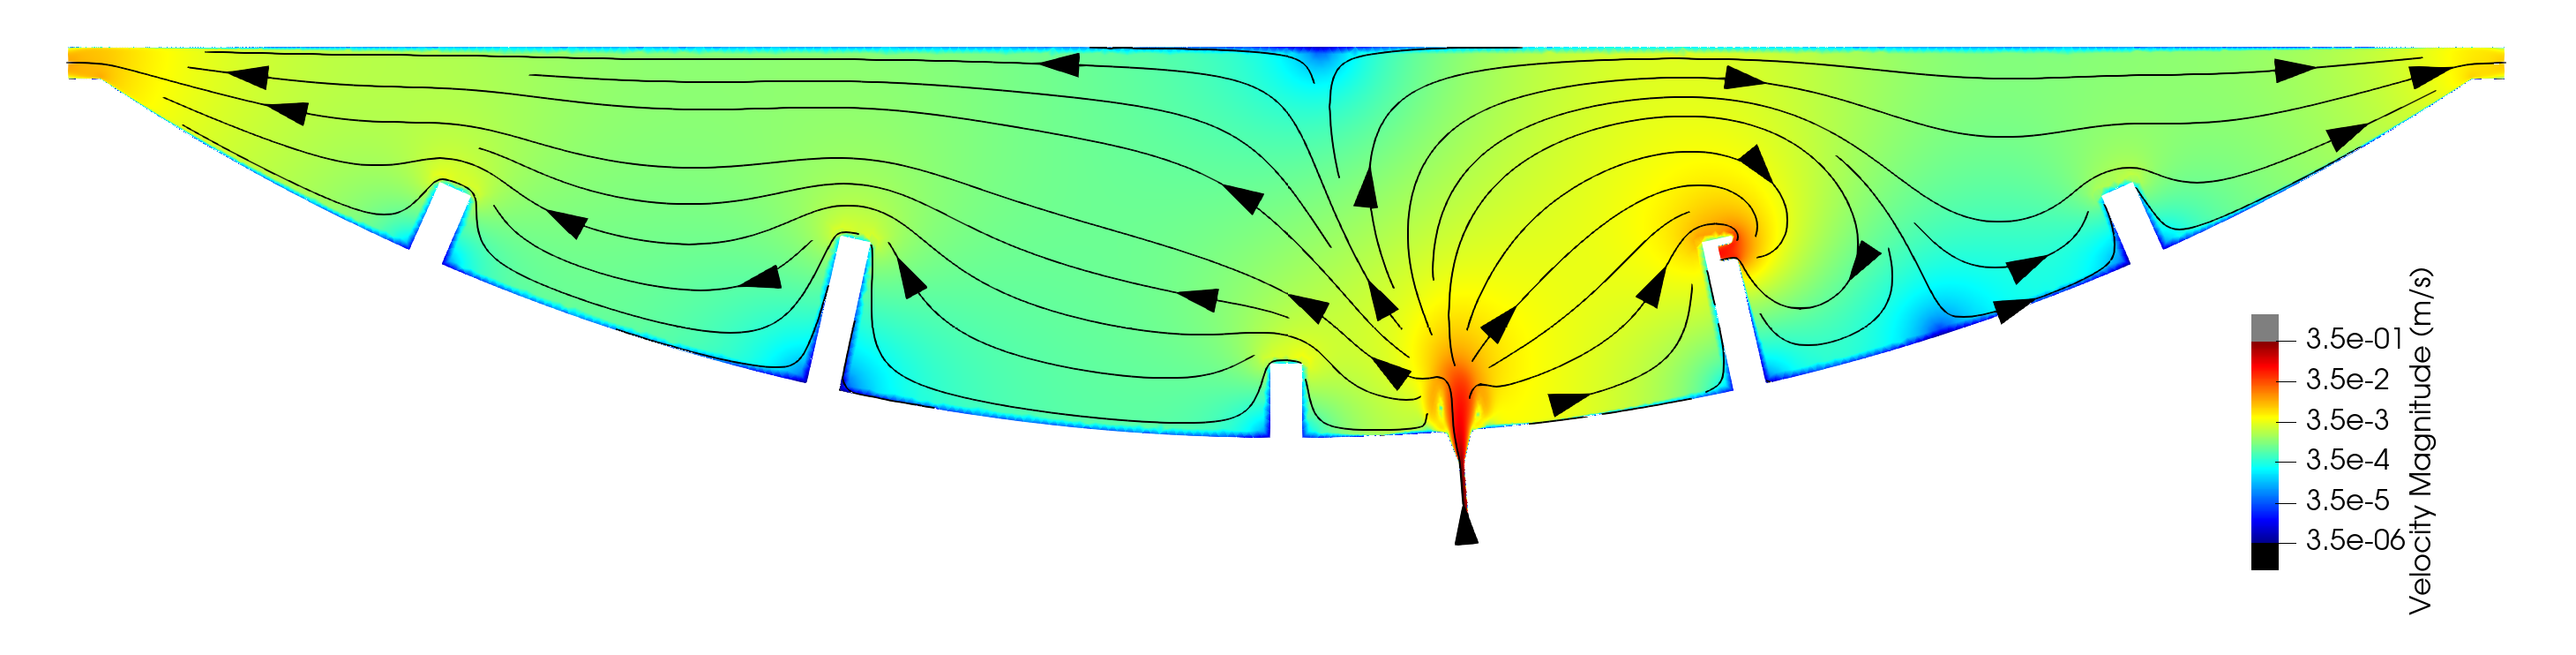
\includegraphics[width=181.5pt,height=46.12pt]{diagrams/results-variations/70-velocity.png}};
%Image [id:dp3190773005750116] 
\draw (135.01,98.75) node  {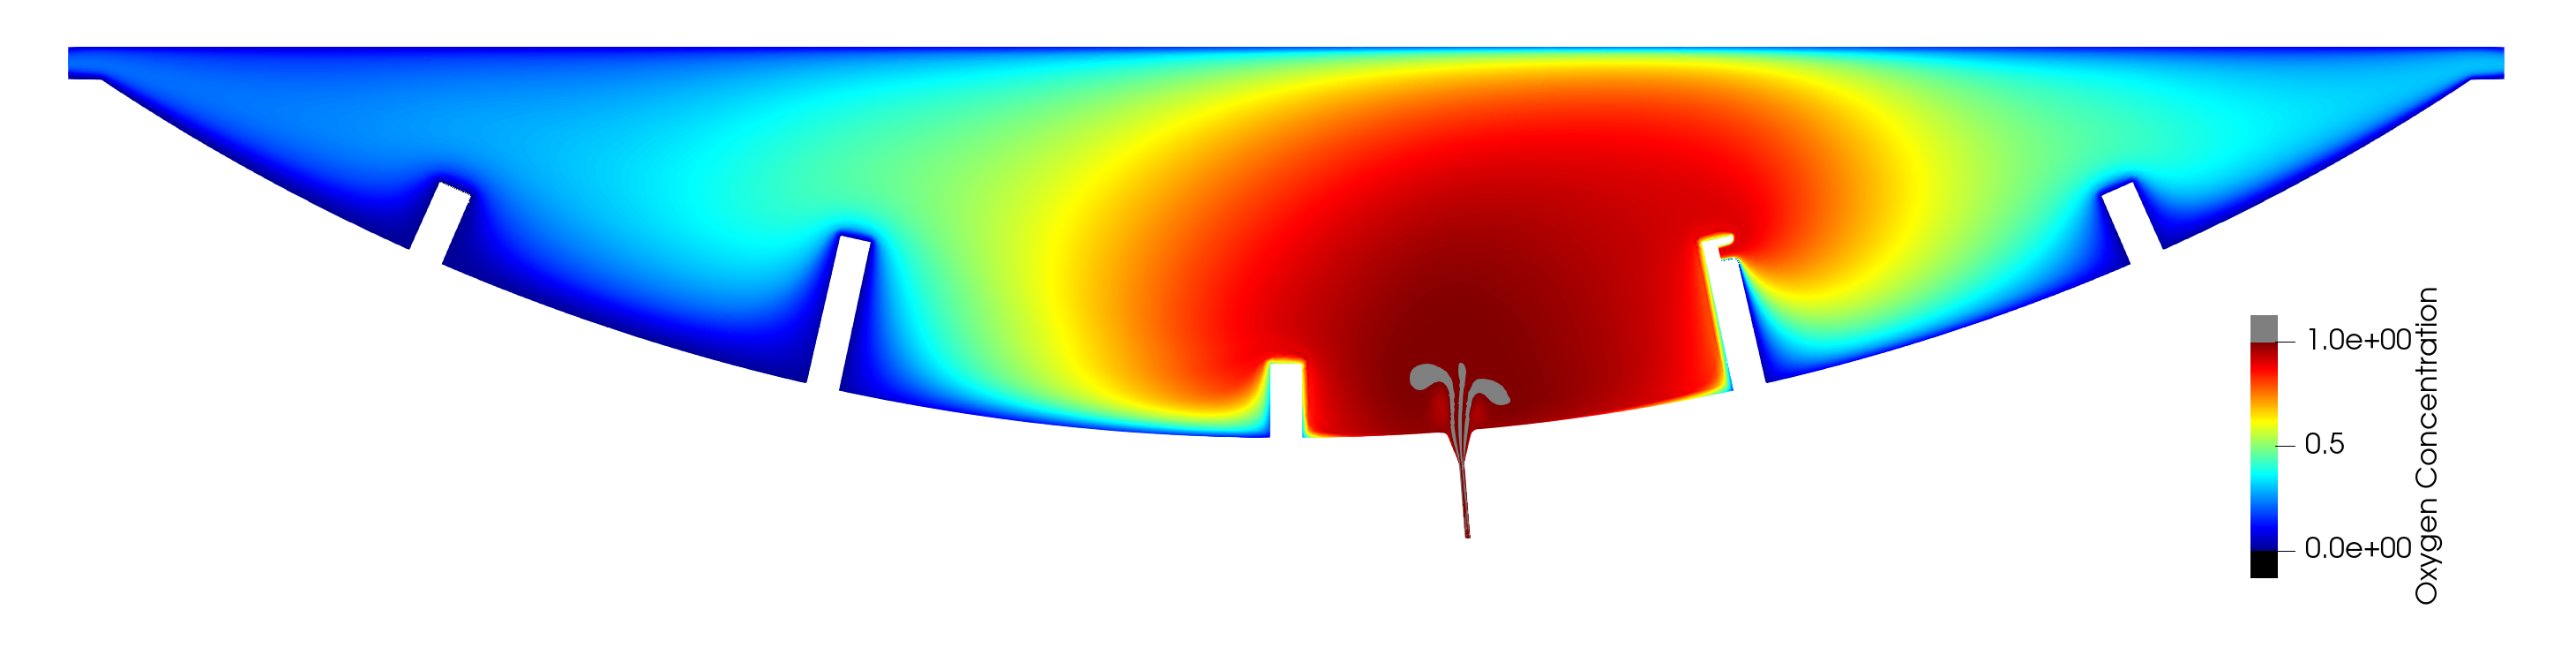
\includegraphics[width=181.52pt,height=46.13pt]{diagrams/results-variations/70-oxygen.png}};
%Image [id:dp5209728544208736] 
\draw (462,43.25) node  {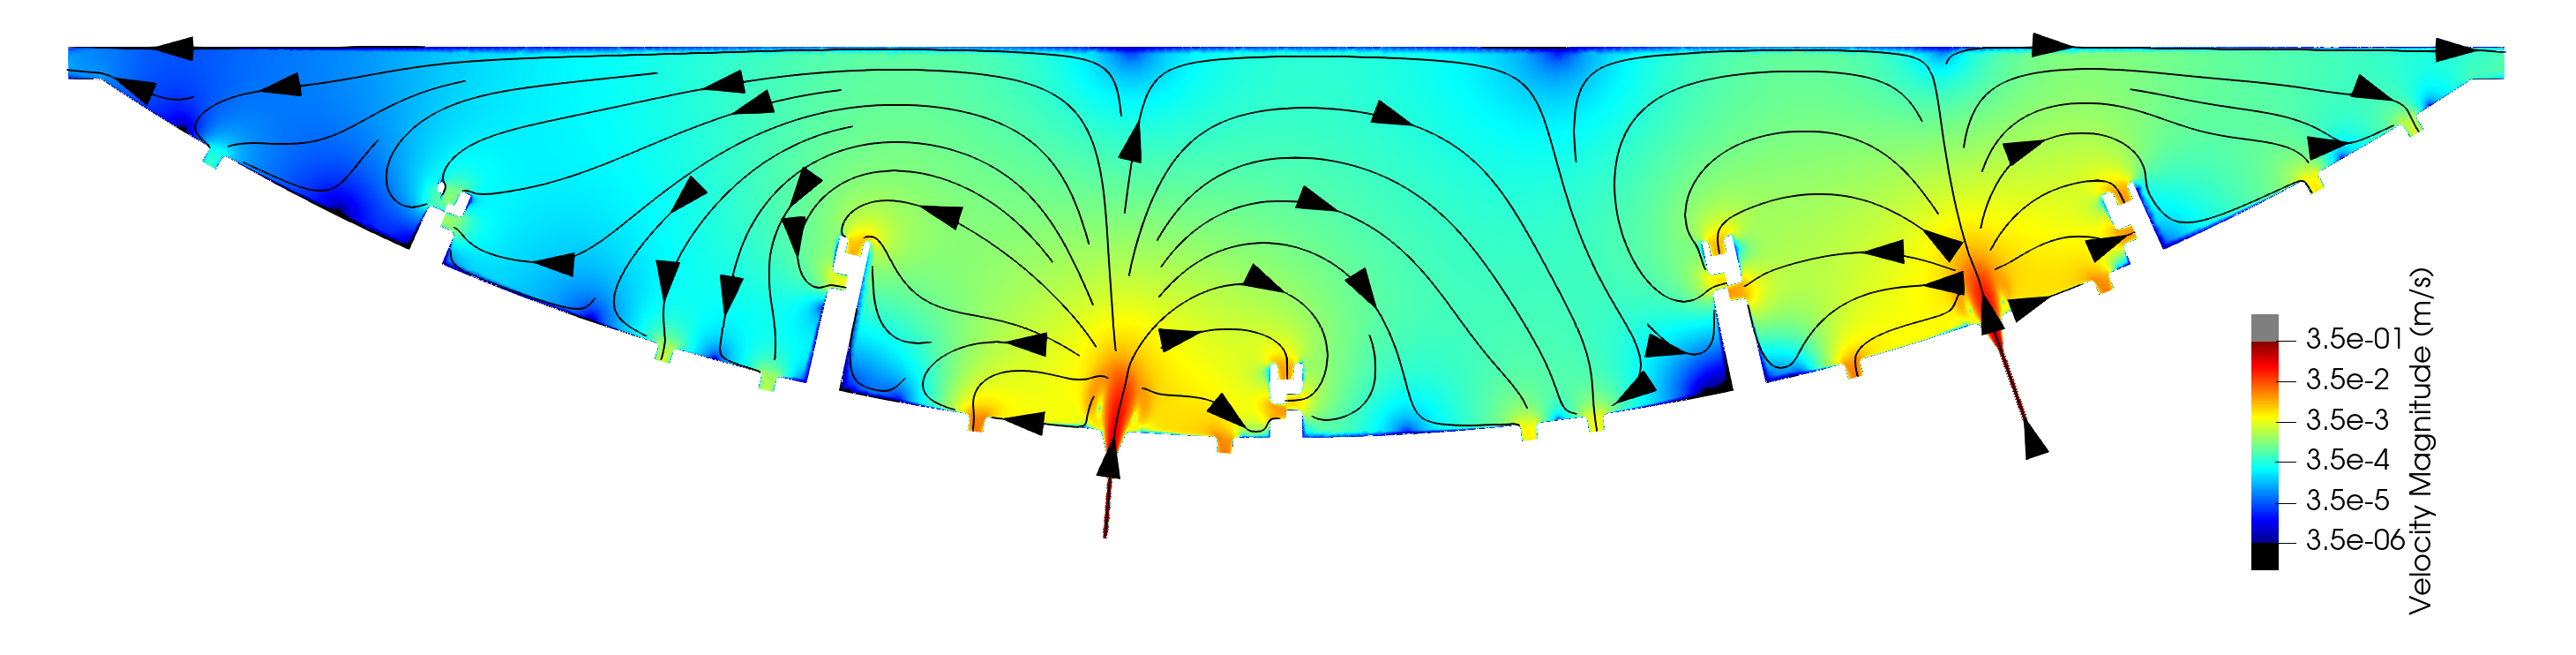
\includegraphics[width=181.5pt,height=46.12pt]{diagrams/results-variations/444-velocity.png}};
%Image [id:dp17912691189229846] 
\draw (461.51,98.25) node  {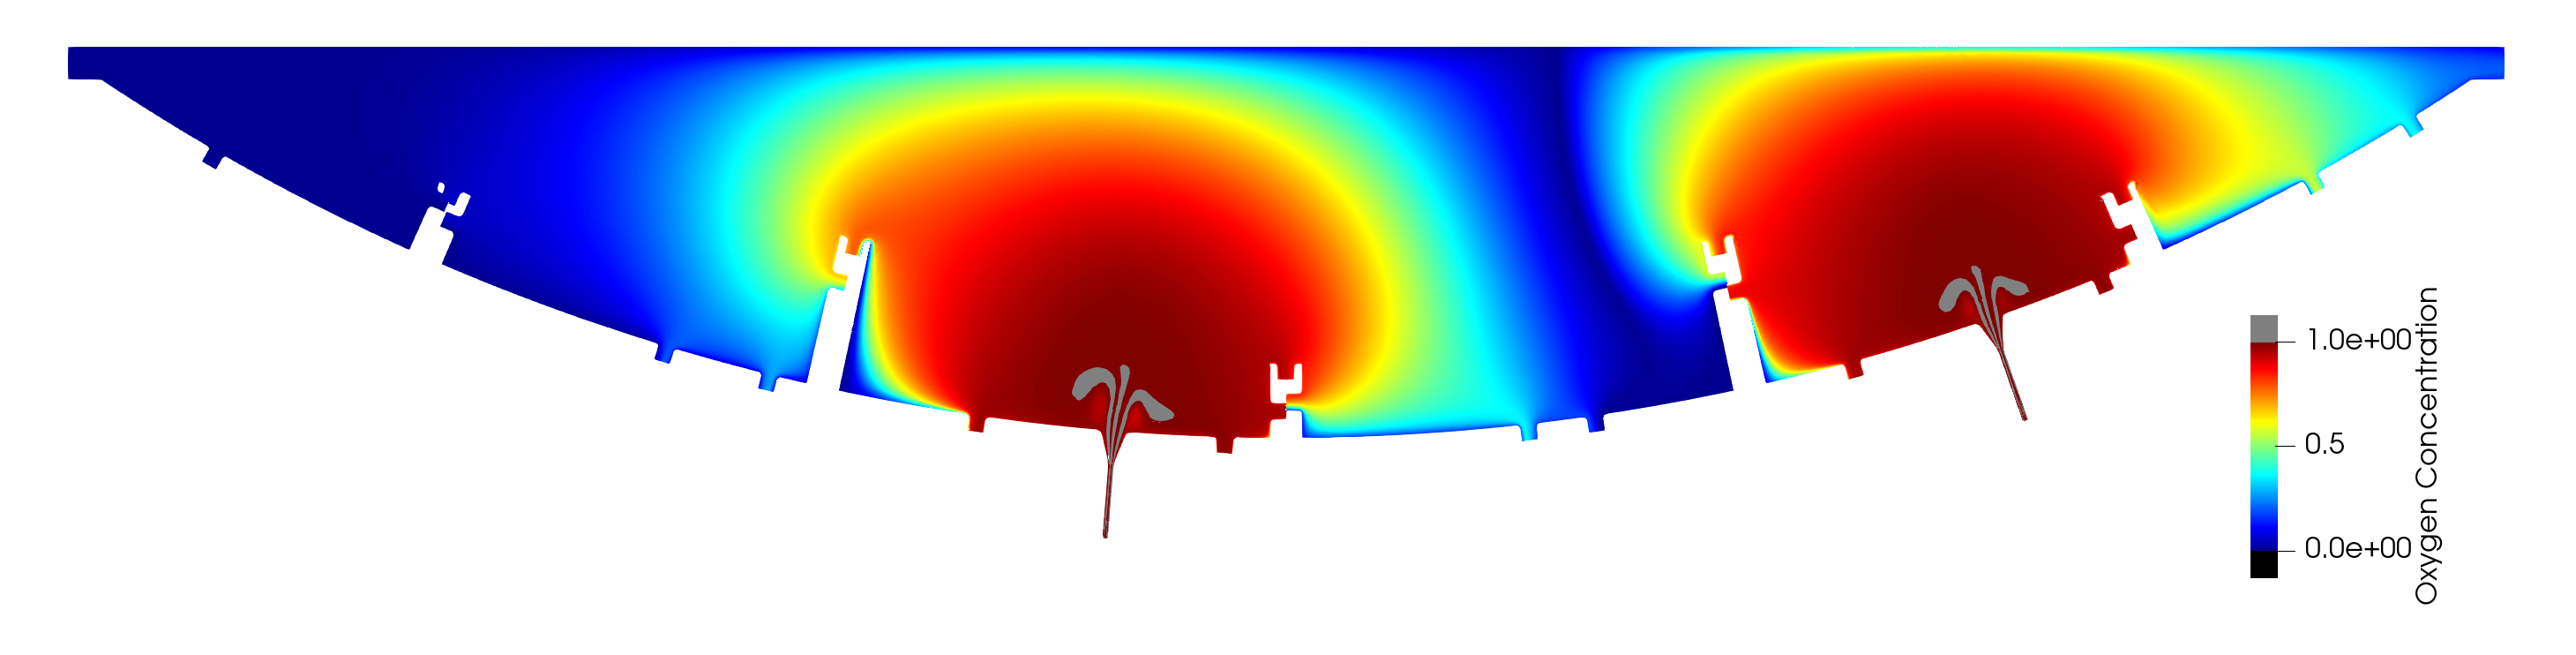
\includegraphics[width=181.52pt,height=46.13pt]{diagrams/results-variations/444-oxygen.png}};
%Image [id:dp7793537016904728] 
\draw (136,169.75) node  {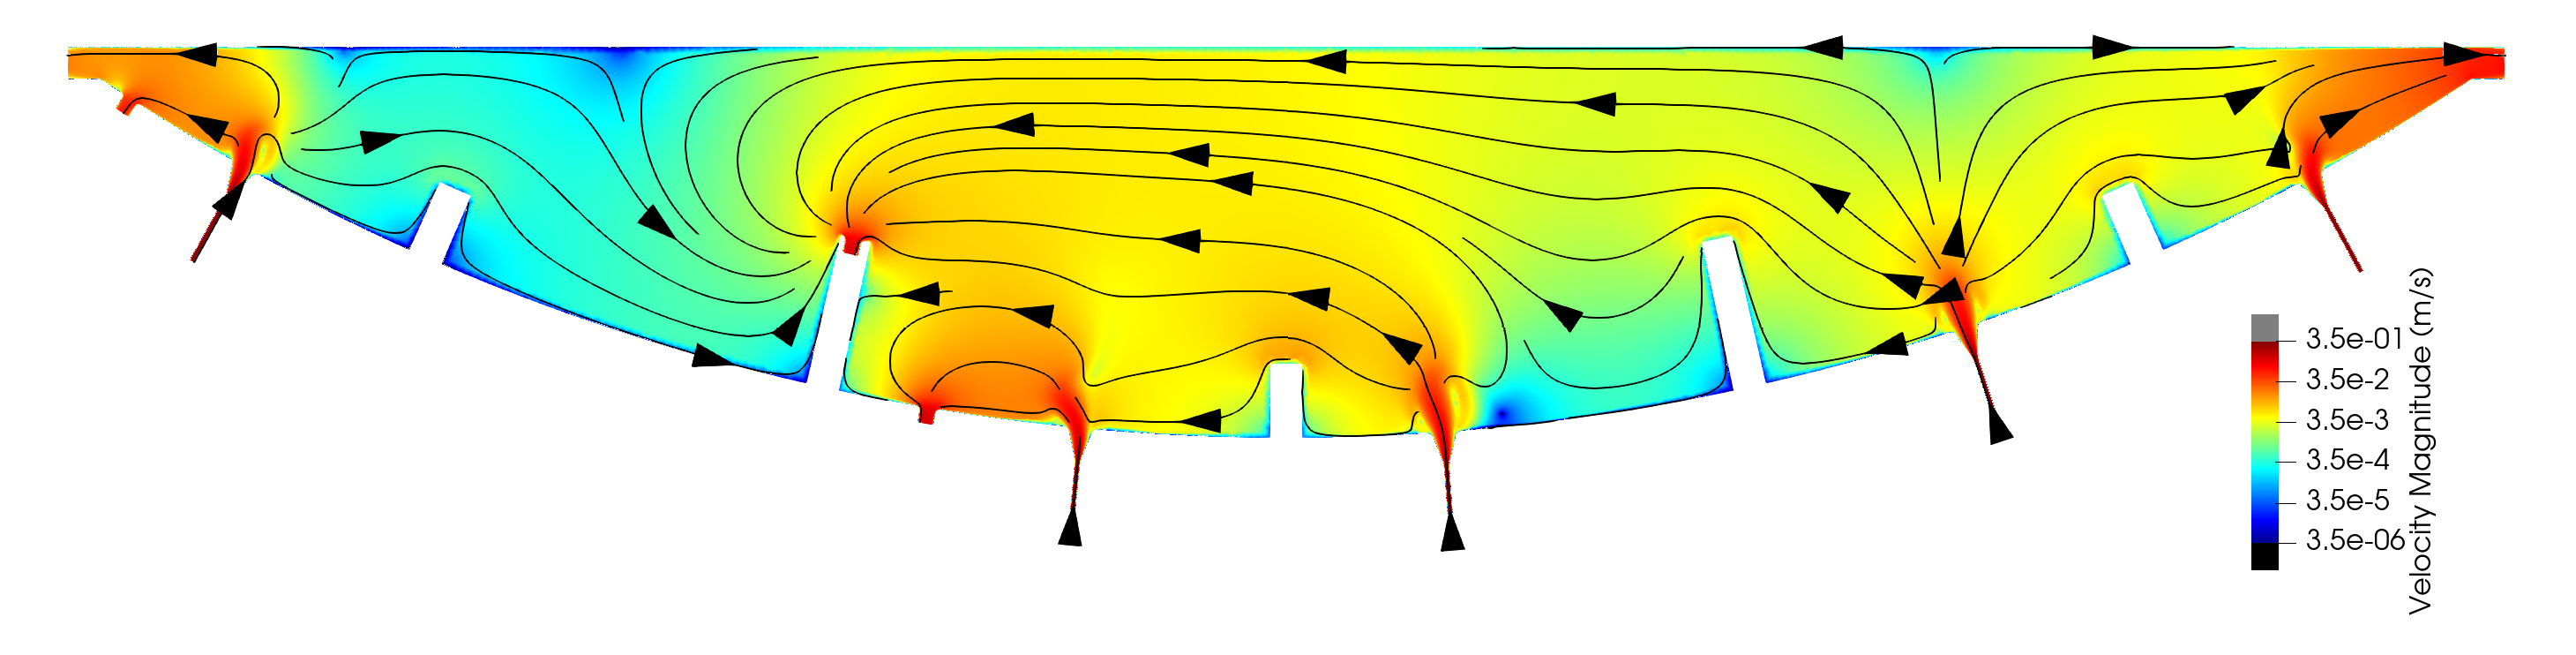
\includegraphics[width=181.5pt,height=46.12pt]{diagrams/results-variations/122-velocity.png}};
%Image [id:dp12012060465786312] 
\draw (135.51,224.75) node  {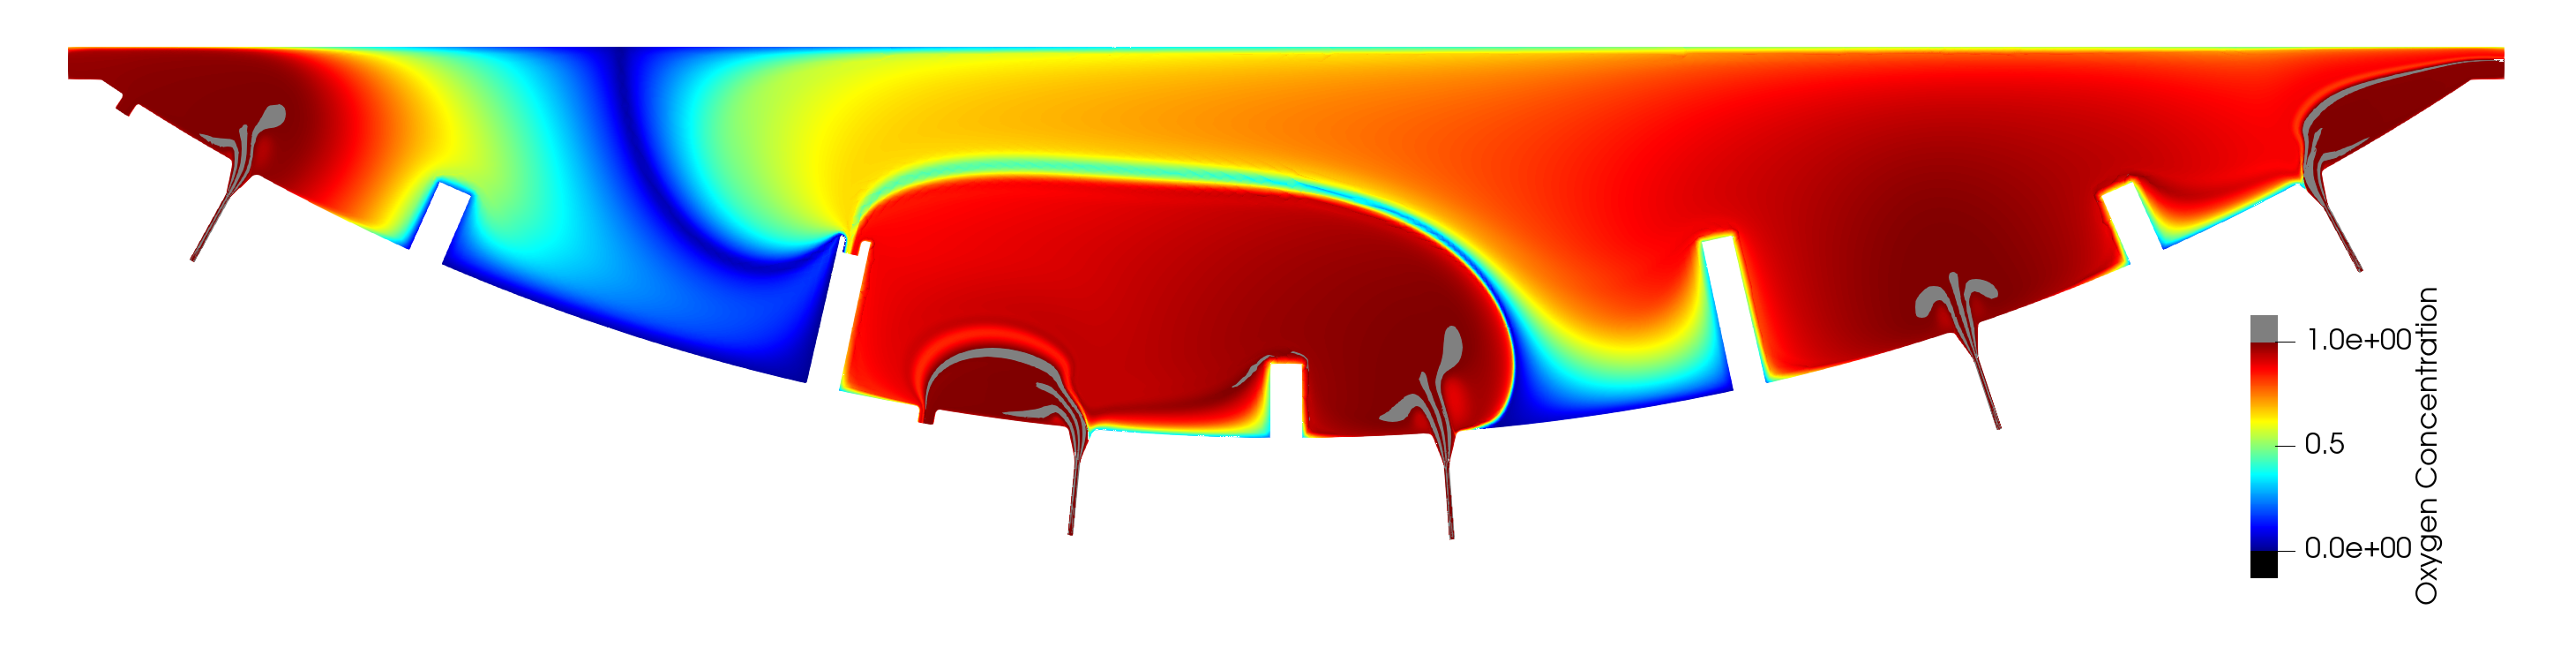
\includegraphics[width=181.52pt,height=46.13pt]{diagrams/results-variations/122-oxygen.png}};
%Image [id:dp8850565235206664] 
\draw (462.5,169.25) node  {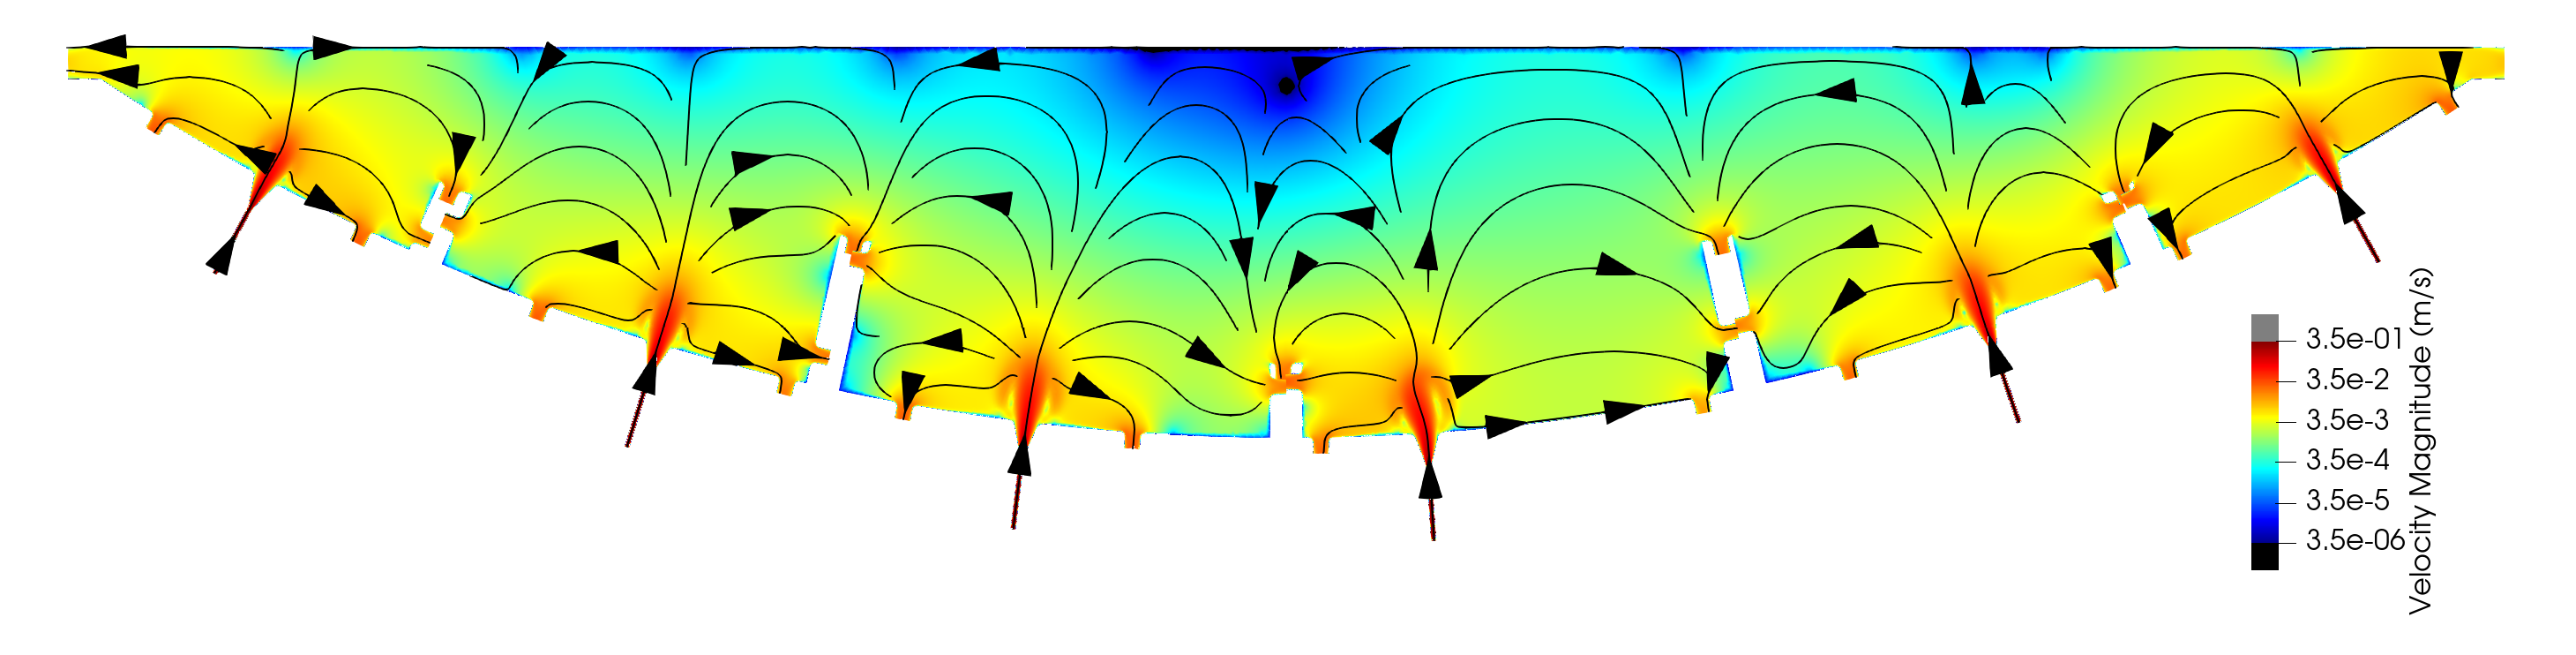
\includegraphics[width=181.5pt,height=46.12pt]{diagrams/results-variations/90-velocity.png}};
%Image [id:dp16362593587874552] 
\draw (462.01,224.25) node  {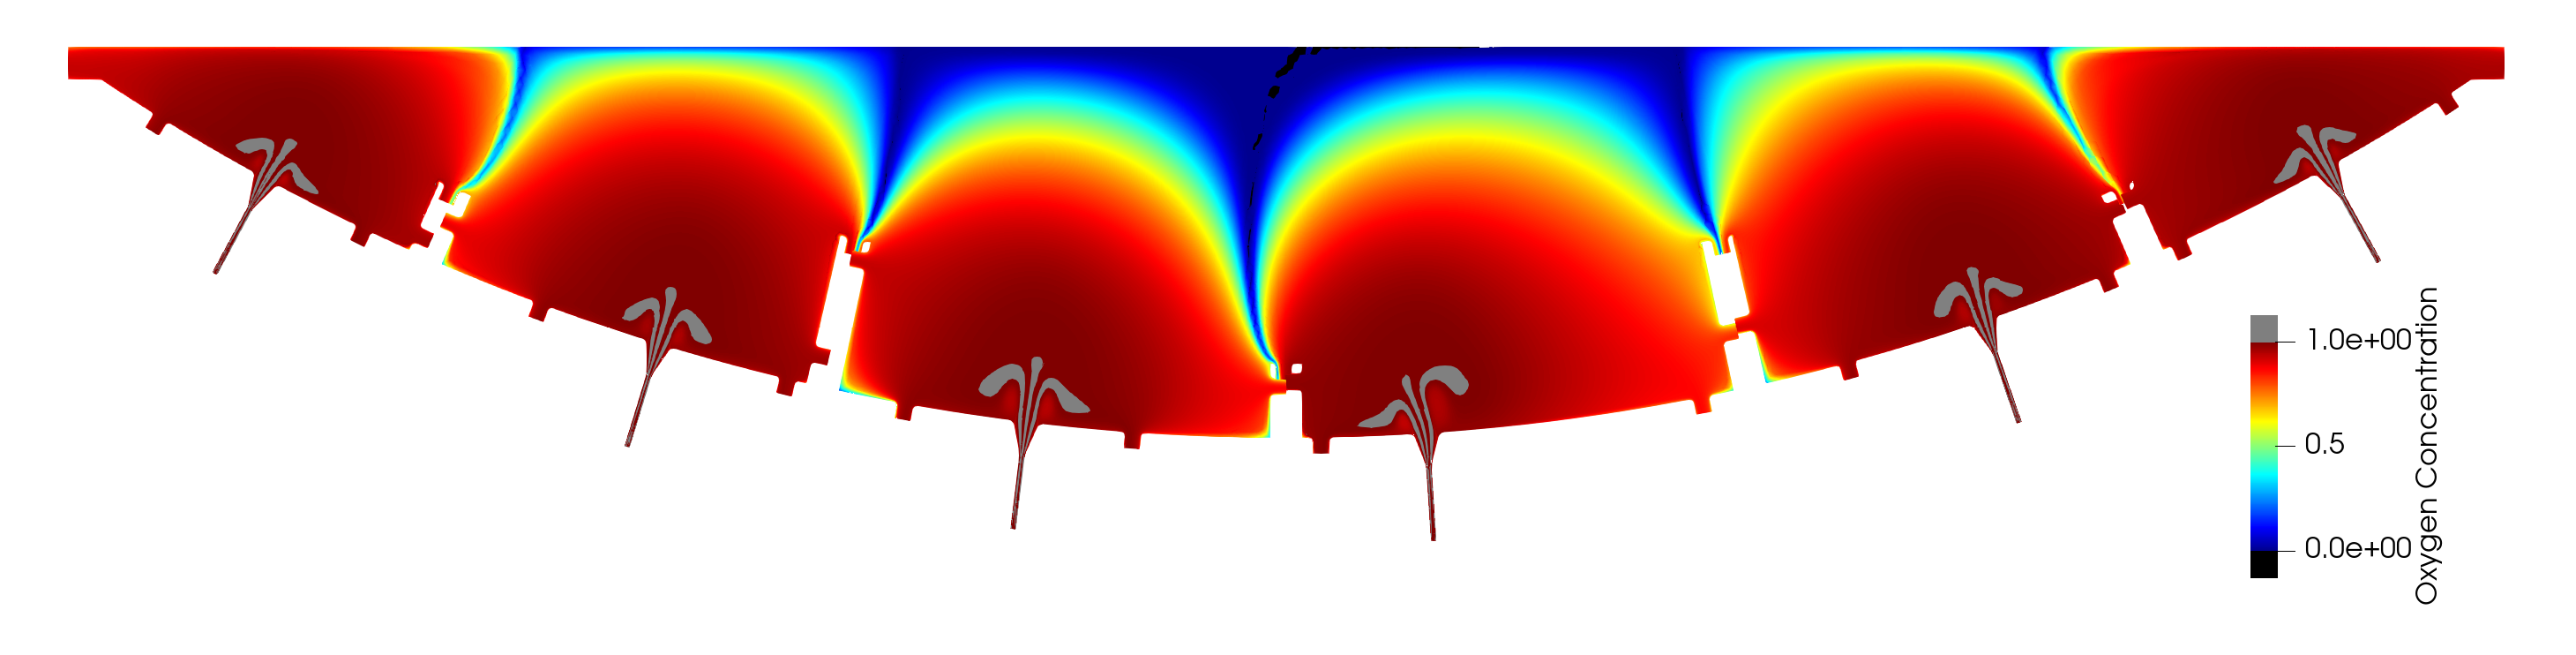
\includegraphics[width=181.52pt,height=46.13pt]{diagrams/results-variations/90-oxygen.png}};

% Text Node
\draw (258.42,70.43) node [anchor=west] [inner sep=0.75pt]    {$ \begin{array}{l}
N_{\text{A}} =1\\
N_{\text{V}} =1
\end{array}$};
% Text Node
\draw (584.92,69.93) node [anchor=west] [inner sep=0.75pt]    {$ \begin{array}{l}
N_{\text{A}} =2\\
N_{\text{V}} =24
\end{array}$};
% Text Node
\draw (258.92,196.43) node [anchor=west] [inner sep=0.75pt]    {$ \begin{array}{l}
N_{\text{A}} =5\\
N_{\text{V}} =3
\end{array}$};
% Text Node
\draw (585.42,195.93) node [anchor=west] [inner sep=0.75pt]    {$ \begin{array}{l}
N_{\text{A}} =6\\
N_{\text{V}} =27
\end{array}$};


\end{tikzpicture}
